%\vspace{-0.1cm}
\section{SiSEC Evaluation Campaigns}
\label{sec:evaluation}

\subsection{Organisation and Open Source Tools}
\label{ssec:background}

The problem of evaluating the quality of audio signals is a research topic of its own, which is deeply connected to psychoacoustics~\cite{zwicker13} and has many applications in engineering because it provides an objective function to optimize when designing processing methods. While mean squared error (MSE) is often used for mathematical convenience whenever an error is to be computed, it is a very established fact that MSE is not representative of audio perception~\cite{rix01,wang09}. For example, inaudible phase shifts would dramatically increase the MSE. Moreover, it should be acknowledged  that the concept of quality is rather application-dependent.

In the case of signal separation or enhancement, processing is often only a part of a whole architecture and a relevant methodology for evaluation is to study the positive or negative impact of this module on the overall performance of the system, rather than to consider it independently from the rest. For example, when embedded in an automatic speech recognition (ASR) system, performance of speech denoising can be assessed by checking whether it decreases word error rate~\cite{barker15}.

When it comes to music processing, and more particularly to lead and accompaniment separation, the evaluation of separation quality has traditionally been inspired by work in the audio coding community~\cite{recommendation2001MUSHRA,rix01} in the sense that it aims at comparing ground truth vocals and accompaniment with their estimates, just like audio coding compares the original with the compressed signal.

%\vspace{-0.2cm}
\subsection{Metrics}
\label{ssec:metrics}

As noted previously, MSE-based error measures are not perceptually relevant. For this reason, a natural approach is to have humans do the comparison. The gold-standard for human perceptual studies is the MUlti Stimulus test with Hidden Reference and Anchor (MUSHRA) methodology, that is commonly used for evaluating audio coding~\cite{recommendation2001MUSHRA}.

However, it quickly became clear that the specific evaluation of separation quality cannot easily be reduced to a single number, even when achieved through actual perceptual campaigns, but that quality rather depends on the application considered. For instance, karaoke or vocal extraction come with opposing trade-offs between isolation and distortion. For this reason, it has been standard practice to provide different and complementary metrics for evaluating separation that measure the amount of distortion, artifacts, and interference in the results.

While human-based perceptual evaluation is definitely the best way to assess separation quality~\cite{vincent062,cano11}, having computable objective metrics is desirable for several reasons. First, it allows researchers to evaluate performance without setting up costly and lengthy perceptual evaluation campaigns. Second, it permits large-scale training for the fine-tuning of parameters. In this respect, the Blind Source Separation Evaluation (BSS Eval) toolbox~\cite{fevotte05a,vincent06} provides quality metrics in decibel to account for distortion (SDR), artifacts (SAR), and interferences (SIR). Since it was made available quite early and provides somewhat reasonable correlation with human perception in certain cases \cite{fox07,fox072} it is still widely used to this day.

Even if BSS Eval was considered sufficient for evaluation purposes for a long time, it is based on squared error criteria. Following early work in the area~\cite{kornycky08}, the Perceptual Evaluation of Audio Source Separation (PEASS) toolkit \cite{emiya10,emiya11,vincent122} was introduced as a way to predict perceptual ratings. While the methodology is very relevant, PEASS however was not widely accepted in practice. We believe this is for two reasons. First, the proposed implementation is quite computationally demanding. Second, the perceptual scores it was designed with are more related to speech separation than to music.
%Derry: Do we have space to add references to work which shows that PEASS fails to correlate with perception for many separation tasks?

Improving perceptual evaluation often requires a large amount of experiments, which is both costly and requires many expert listeners. One way to increase the number of participants is to conduct web-based experiments. In~\cite{cartwright16}, the authors report they were able to aggregate 530 participants in only 8.2 hours and obtained perceptual evaluation scores comparable to those estimated in the controlled lab environment.

Finally, we highlight here that the development of new perceptually relevant objective metrics for singing voice separation evaluation remains an open issue~\cite{gupta15}. It is also a highly crucial one for future research in the domain.

\subsection{Results SiSEC 2015}
\label{ssec:performance}

\kant[1-16]

%\vspace{-0.2cm}
\subsection{Results SiSEC 2016}
\label{ssec:performance}

In this section, we will discuss the performance of $23$ source separation methods evaluated on the DSD100, as part of the task for separating professionally-produced music recordings at SiSEC 2016. The methods are listed in Table~\ref{tab:systems}, along with the acronyms we use for them, their main references, a very brief summary, and a link to the section where they are described in the text. To date, this stands as the largest evaluation campaign ever achieved on lead and accompaniment separation. The results we discuss here are a more detailed report for SiSEC~2016~\cite{liutkus17}, presented in line with the taxonomy proposed in this paper.

\begin{table}[htbp]
	\centering
	\caption{Methods evaluated during SiSEC 2016.}
	\label{tab:systems}
	\begin{tabular}{|lll@{}l@{}|}
		\hline
		\textbf{Acronym} & \textbf{Ref.} & \textbf{Summary} & \textbf{Section}\\
		\hline
		HUA & \cite{huang12} & RPCA standard version & \ref{ssec:RPCA}\\
		\hline
		RAF1 & \cite{rafii13} & REPET standard version & \ref{ssec:methods_repet}\\
		RAF2 & \cite{liutkus12} & REPET with time-varying period & \\
		RAF3 & \cite{rafii12} & REPET with similarity matrix & \\
		KAM1-2 & \cite{liutkus15} & KAM with different configurations &\\
		\hline
		CHA & \cite{chan15} & RPCA with vocal activation information &\ref{ssec:methods_structureinformed}\\
		JEO1-2 & \cite{jeong17} &  $l_1$-RPCA with vocal activation information &\\
		\hline
		DUR & \cite{durrieu11} & Source-filter NMF &\ref{ssec:methods_sourcefilter}\\
		\hline
		OZE & \cite{salaun14} & Structured NMF with learned dictionaries & \ref{ssec:methods_datadriven_nmf}\\
		\hline
		KON & \cite{huang15} & RNN & \ref{ssec:methods_dnn} \\
		GRA2-3 & \cite{grais16} & DNN ensemble &\\
		STO1-2 & \cite{stoter16} & FNN on \textit{common fate} TF representation&\\
		UHL1 & \cite{Uhlich15} & FNN with context&\\
		\hline
		NUG1-4 & \cite{nugraha16} & FNN with multichannel information &\ref{sec:multichannel}\\
		UHL2-3 & \cite{uhlich17} & LSTM with multichannel information &\\
		\hline
		IBM & & ideal binary mask &  \\
		\hline
	\end{tabular}
\end{table}

%announcing the results and the webpage
The objective scores for these methods were obtained using BSS Eval and are given in Figure~\ref{fig:eval}. For more details about the results and for listening to the estimates, we refer the reader to the dedicated interactive website\footnote{\url{http://www.sisec17.audiolabs-erlangen.de}}.

\begin{figure*}[htbp]
	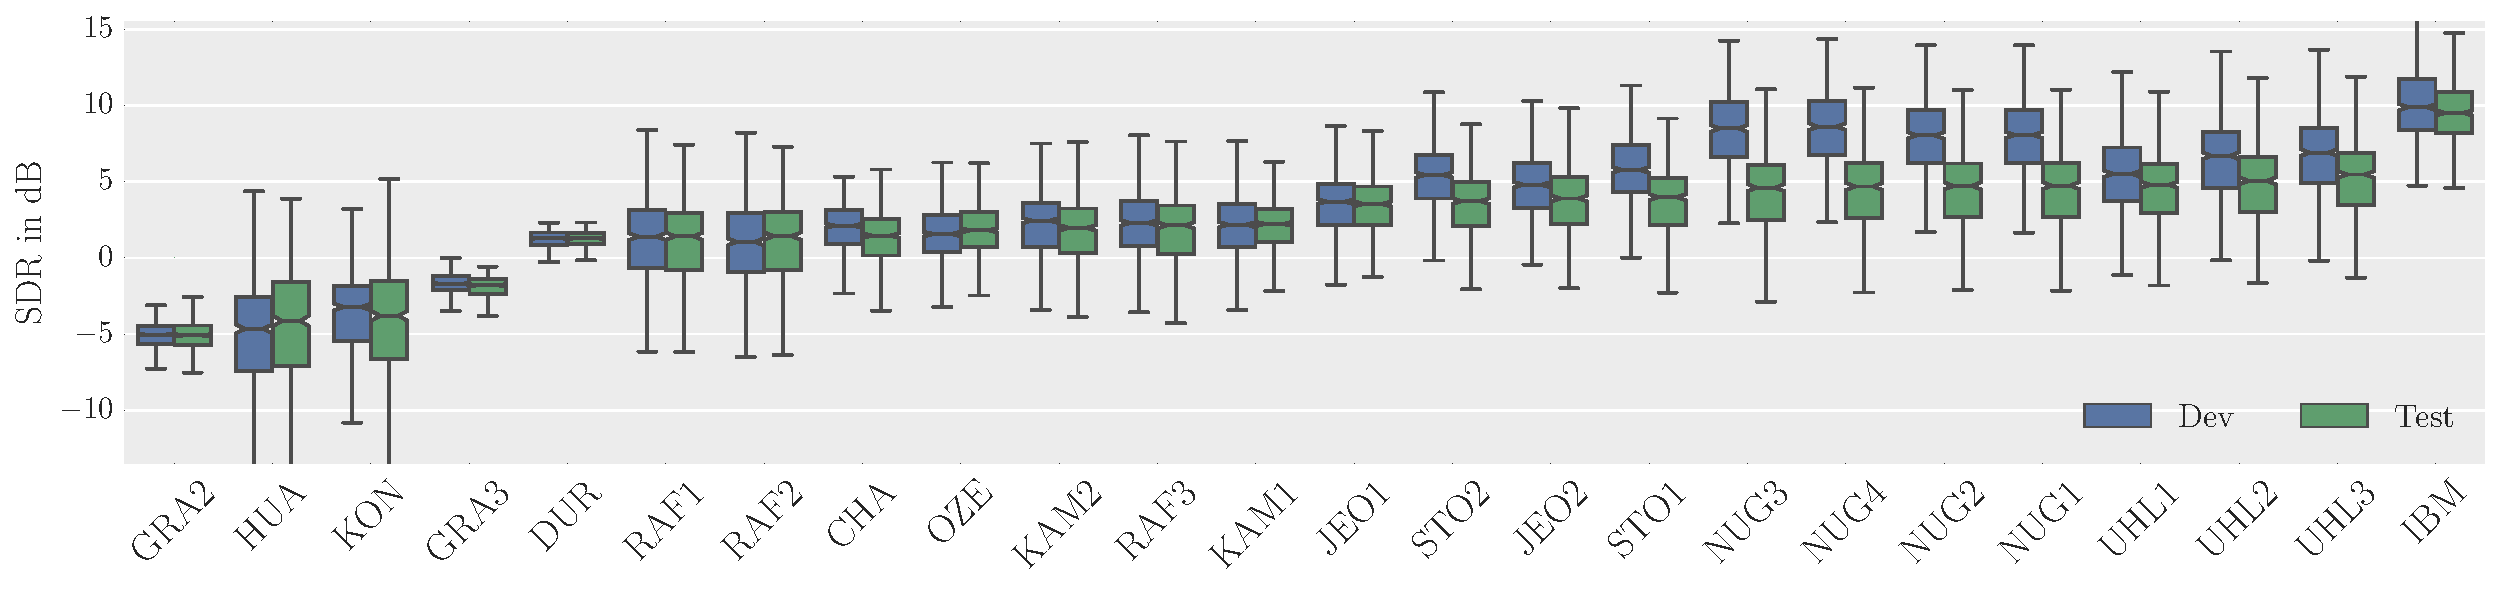
\includegraphics[width=\textwidth]{gfx/vocalsSDR.pdf}
	\caption{BSS Eval scores for the vocals and accompaniment estimates for SiSEC 2016 on the DSD100 dataset. Results are  shown for the \emph{test} set only. Scores are grouped as in Table~\ref{tab:systems} according to the section they are described in the text, indicated below each group.}
	\label{fig:eval}
\end{figure*}

%RPCA suffers from full-length recordings
As we first notice in Figure~\ref{fig:eval}, the HUA method, corresponding to the standard RPCA as discussed in Section~\ref{ssec:RPCA}, showed rather disappointing performance in this evaluation. After inspection of the results, it appears that processing full-length tracks is the issue there: at such scales, vocals also exhibit redundancy, which is captured by the low-rank model associated with the accompaniment. On the other hand, the RAF1-3 and KAM1-3 methods that exploit redundancy through repetitions, as presented in Section~\ref{ssec:methods_repet}, behave much better for full-length tracks: even if somewhat redundant, vocals are rarely as repetitive as the accompaniment. When those methods are evaluated on datasets with very short excerpts (e.g., MIR-1K), such severe practical drawbacks are not apparent.

%DUR also+non harmonic lead
Likewise, the DUR method that jointly models the vocals as harmonic and the accompaniment as redundant, as discussed in Section~\ref{ssec:methods_sourcefilter}, does show rather disappointing performance, considering that it was long the state-of-the-art in earlier SiSECs \cite{vincent12}. After inspection, we may propose two reasons for this performance drop. First, using full-length excerpts also clearly revealed a shortcoming of the approach: it poorly handles silences in the lead, which were rare in the short-length excerpts tested so far. Second, using a much larger evaluation set revealed that vocals are not necessarily well modeled by a harmonic source-filter model; breathy or saturated voices appear to greatly challenge such a model.

%RPCA informed by lead presence behaves well
While processing full-length tracks comes as a challenge, it can also be an opportunity. It is indeed worth noticing that whenever RPCA is helped through vocal activity detection, its performance is significantly boosted, as highlighted by the relatively good results obtained by CHAN and JEO.

%OZE could benefit from the new learning data
As discussed in Section~\ref{sec:datadriven-approaches}, the availability of learning data made it possible to build data-driven approaches, like the NMF-based OZE method which is available through the Flexible Audio Source Separation Toolbox (FASST) \cite{salaun14,ozerov12}. Although it was long state-of-the-art, it has been strongly outperformed recently by other data-driven approaches, namely DNNs. One first reason clearly appears as the superior expressive power of DNNs over NMF, but one second reason could very simply be that OZE should be trained anew with the same large amount of data.

%DNN are definitely performing awesomely
As mentioned above, a striking fact we see in Figure~\ref{fig:eval} is that the overall performance of data-driven DNN methods is the highest. This shows that exploiting learning data does help separation greatly compared to only relying on \textit{a priori} assumptions such as the harmonicity or redundancy. Additionally, dynamic models such as CNN or LSTM appear more adapted to music than FNN. These good performances in audio source separation go in line with the recent success of DNNs in fields as varied as computer vision, speech recognition, and natural language processing \cite{lecun15}.

%but it's clear that they benefit from smart ideas
However, the picture may be seen to be more subtle than simply black-box DNN systems beating all other approaches. For instance, exploiting multichannel probabilistic models, as discussed in Section~\ref{sec:multichannel}, leads to the NUG and UHL2-3 methods, that significantly outperform the DNN methods ignoring stereo information. In the same vein, we expect other specific assumptions and musicological ideas to be exploited for further improving the quality of the separation.

%weakness of metrics
One particular feature of this evaluation is that it also shows obvious weaknesses in the objective metrics. For instance, the GRA method behaves significantly worse than any other methods. However, when listening to the separated signals, this does not seem deserved. All in all, designing new and convenient metrics that better match perception and that are specifically built for music on large datasets clearly appears as a desirable milestone.

%IBM much better: room for improvement
In any case, the performance achieved by a totally informed filtering method such as IBM is significantly higher than that of any submitted method in this evaluation. This means that lead and accompaniment separation has room for much improvement, and that the topic is bound to witness many breakthroughs still. This is even more true considering that IBM is not the best upper bound for separation performance: other filtering methods such as \textit{ideal ratio mask}~\cite{liutkus15c} or multichannel Wiener filter~\cite{duong10} may be considered as references.

%importance of implementations and details, links to online ressources
Regardless of the above, we would also like to highlight that good algorithms and models can suffer from slight errors in their low-level audio processing routines. Such routines may include the STFT representation, the overlap-add procedure, energy normalization, and so on. Considerable improvements may also be obtained by using simple tricks and, depending on the method, large impacts can occur in the results by only changing low-level parameters. These include
%the length of each window, S: I think that this is not a trick. Various window sizes lead to different representations (sparser/disjoint) and they are a part of modelling the data. I believe we should keep it out.
the overlap ratio for the STFT, specific ways to regularize matrix inverses in multichannel models, etc. Further tricks such as the exponentiation of the TF mask by some positive value can often boost performance significantly more than using more sophisticated models. However, such tricks are often lost when publishing research focused on the higher-level algorithms. We believe this is an important reason why sharing source code is highly desirable in this particular application. Some online repositories containing implementations of lead and accompaniment separation methods should be mentioned, such as \textbf{nussl}\footnote{\url{https://github.com/interactiveaudiolab/nussl}} and \textbf{untwist} \cite{roma16}. In the companion webpage of this paper\footnote{\url{https://sigsep.github.io}}, we list many different online resources such as datasets, implementations, and tools that we hope will be useful to the practitioner and provide some useful pointers to the interested reader.
